\subsubsection{Presentation}
Support Vector Machines are a model of supervised learning.\\
In summary, the model finds the hyperplane (kernel) that maximizes the Margin of Safety for classifying.

\subsubsection{Defining Parameters}
The data for training and validating is already defined by the Data Preparation step (80\% train, 20\% validation).\\
Representative parameters for the model are \emph{gamma} and \emph{C}
\begin{itemize}
    \item \underline{gamma}: kernel coefficient
    \item \underline{C}: regularization parameter (higher C, higher variance)
\end{itemize}
We train the following values for the \emph{gamma} parameter: [0.001, 0.01, 0.03, 0.05, 0.08, 0.1, 0.5]
To improve the predictions, we regularize the data using a StandardScaler (removes the mean and scales to unit variance)
The training error and the validation error for each value allow us to plot a Complexity Curve, to select the optimal value fo the parameter.
\begin{center}
    \captionsetup{type=figure}
    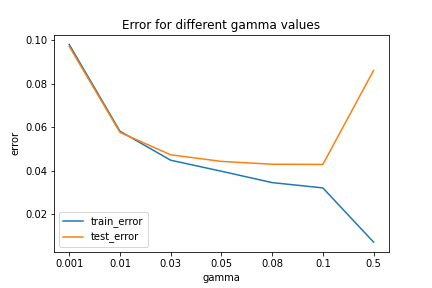
\includegraphics[width=250px]{comp_curve_svm_gamma.png}
    \captionof{figure}{Complexity Curve: \emph{gamma} value for SVM}
\end{center}
By observing the plot, we determine that the best value for gamma is 0.03\\
We train the following values for the \emph{C} parameter: [0.02, 0.2, 0.8, 1.2, 2, 5, 10]\\
Again, we regularize the data using a StandardScaler (removes the mean and scales to unit variance)\\
The training error and the validation error for each value allow us to plot a new Complexity Curve, to select the optimal value fo the parameter.
\begin{center}
    \captionsetup{type=figure}
    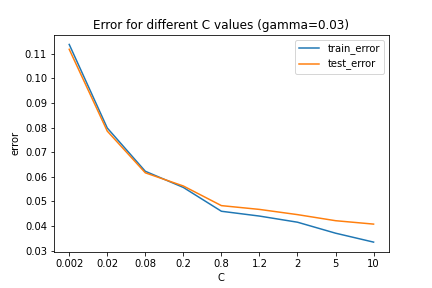
\includegraphics[width=250px]{comp_curve_svm_C.png}
    \captionof{figure}{Complexity Curve: \emph{C} value for SVM (\emph{gamma}=0.03)}
\end{center}
By observing the plot, we determine that the best value for C is 0.8

\subsubsection{Model Evaluation}
Chosen the parameters: (\emph{gamma}=0.03, \emph{C}=0.8), a learning curve shows us the training and validation scores for different data sizes.\\
This way, we are able to say that the score is bounded below 95\%, and the model doesn't seem to continue learning after 65000/70000 training rows.
\begin{center}
    \captionsetup{type=figure}
    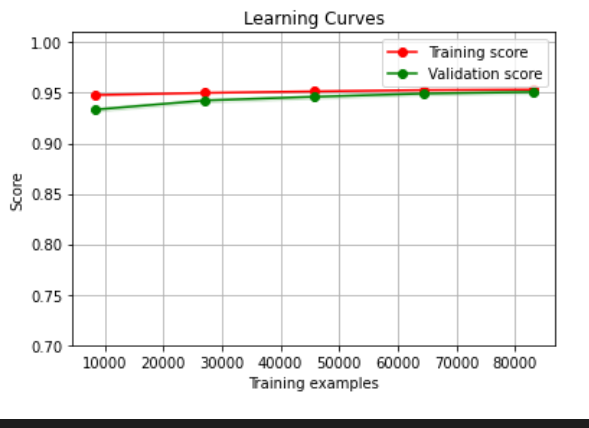
\includegraphics[width=250px]{learning_curve_svm.png}
    \captionof{figure}{Learning Curve for SVM}
\end{center}
